
\chapter{大脑和思维}

\section{关于思维的新观点}

只是随着计算机的出现,人们才真正试图制造“能思维的”机器,并见识了思维这个主题上各种稀奇古怪的变奏。一些程序设计出来了,但若把它们的“思维”与人的思维相比,那就如同把鹦鹉的叽喳学舌与人说话相比一样。这种新发现出来的能力,即用具有与人类完全不同的、但却是人工构造的思维形式——或思维的近似物——来做实验的能力,突然之间揭示出了人类思维的特性、缺陷、威力、捉摸不定之处和发展变化之道。结果是近二十年来,我们在关于思维是什么、不是什么这一问题上,获得了一些新的观点。与此同时,脑的研究者们对于大脑硬件的小尺度及大尺度的探索也都大有收获。这种探索目前还不足以清楚地揭示出脑是如何处理概念的,但已使我们对思维过程所凭藉的生物机制有了一些认识。

在下面两章中,我们将努力把几个领域的研究成果结合起来,包括实现计算机智能的尝试、在活的动物脑上所做的精巧实验以及认知心理学家对人的思维过程的探索。《前奏曲,蚂蚁赋格》已经为此做了铺垫,现在我们来进一步展开其中的观点。

\section{内涵与外延}

思维必须依赖于在大脑硬件中对客观实在的表示。在前面几章中,我们已经开发了几个形式系统,数学实在的领域可以在那种符号体系中表示出来。用这样的形式系统作为大脑如何支配思想的模型,在多大程度上是合理的?

在pq系统以及后来的几个更复杂的系统中,我们已经看到了意义——在这个词的受到一定限制的意思下——是如何作为一种同构的结果而出现的。这种同构把印刷符号映射到数、运算和关系,把印刷符号串映射到陈述。在大脑中我们没有印刷符号,但我们有更好的东西:能动的成分,它们可以存贮、传送并从其它能动成分接收信息。也就是说,我们有主动的符号,而不是被动的印刷符号。在大脑中,规则就混在这些符号之内(而在纸上,符号是静止实体,规则是在我们的头脑里)。

要强调的一点是:从我们已经见到的那些形式系统所具有的相当严格的性质中不应产生这样的想法:符号与现实事物之间的同构是刻板的一一映射,就像木偶与牵着它的那根线一样。在TNT中,“$50$”这个概念可以有不同的符号表示公式,例如
\[
\begin{gathered}
((SSSSSSS0\cdot SSSSSSS0+(S0\cdot S0))\\
((SSSSS0\cdot SSSSS0)+(SSSSS0\cdot SSSSS0))
\end{gathered}
\]
两者表示同一个数,这一点并不是自明的。你可能分别处理每个表达式,后来在某个时刻你偶然碰上了一个定理,不禁叫道“啊——它就是那个数!”

你的心智同样可能对同一个人有不同的描述,例如
\begin{itemize}
\item 我不久前送给一个在波兰的朋友的那本书的作者。
\item 今晚在这个饭馆里同我和我的朋友聊天的这个陌生人。
\end{itemize}
两者表示同一个人,这一点并不是自明的。这两个描述可能互不相干地存在于你的脑海中。在这个夜晚的某个时刻你们可能偶然谈起了某个话题,由此导致你发现二者指示同一个人,不禁叫道“啊——你就是那个人!”

对于一个人的各种描述并非都要联系于某个存贮着他姓名的中心符号。描述本身就可以被构造和处理。我们可以通过构造一个描述来创造不存在的人;当发现两个描述表示同一实体时,我们可以使它们合为一体;当发现一个描述表示着两个事物时,我们可以把它分成两半——如此等等。这种“描述的演算”存在于思维的核心之中。它被称作是“内涵的”而非“外延的”,意思是描述可以“漂浮”着,而不落实在具体的已知客体上。思维的内涵性与其灵活性相关联,它使我们能够想象假设的世界,合并不同的描述,或把一个描述砍成分离的几段,等等。

假设一个借走了你自行车的朋友打来电话说,她被一辆汽车撞了,你的自行车彻底完蛋了,她也差点一命呜呼。你于是在脑海里想象出一系列场面。随着她不断地添加细节,这些场面越来越生动,到最后你简直就像亲眼见到了一样。然后她告诉你这一切只不过是一个玩笑,她和自行车全都安然无恙!很大程度上这其实无济于事:那个故事和那些场景的生动性丝毫不受影响,而且这段记忆将伴随你很长很长时间。以后,你甚至会由于这一印象的强烈影响而认为她骑车是靠不住的,而这些印象在你得知它们并不真实之后,本应已被抹掉了。幻想和事实在我们的头脑里紧密地混在一起,这是由于思维牵涉到复杂描述的构造和处理,而这些描述并非一定要束缚于真实的事件或物体。

一个关于世界的灵活的内涵表示是思维的全部所在。那么,像脑这样一个生理系统是怎样支持这样一个表示系统的呢?

\section{大脑中的“蚂蚁”}

\begin{figure}
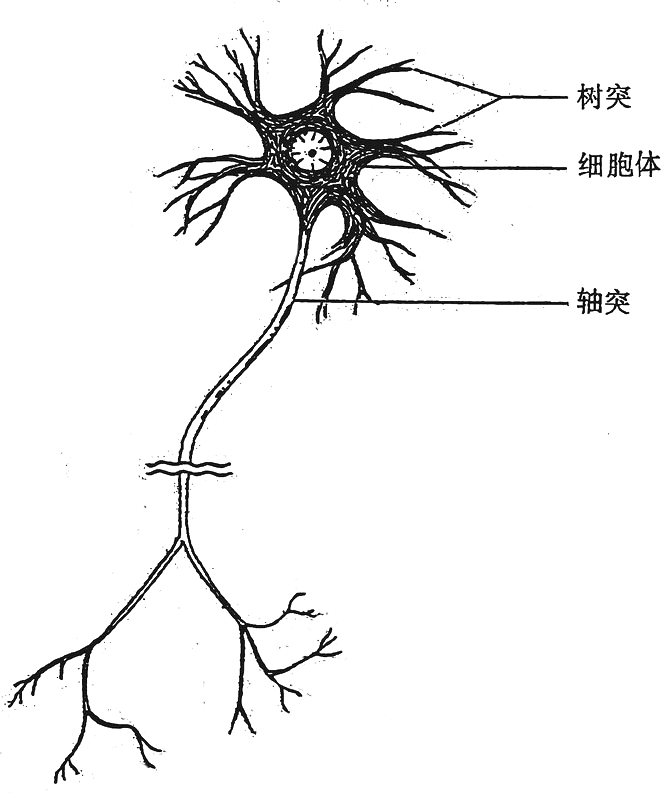
\includegraphics{img_065.png}
\caption[神经元示意图。]
  {神经原示意图[摘自伍尔德里奇[D.Wooldridge],《大脑的机制》[\bn{The Machinery of the Brain}],纽约:Mc-Graw-Hill,1963年版,第6页。] }
\end{figure}

大脑中最为重要的细胞是神经细胞,或称神经元(见\fig{65}),它们大约有一百亿个(奇怪的是,胶质细胞的数目是神经元的十倍。据信,它们主要是对神经元这个主角起支持作用的,因此我们这里不讨论它们)。每个神经元具有若干个突触(“输入端口”)和一个轴突(“输出通道”)。输入和输出均为电化学流,即移动的离子。神经元的输入端口和输出通道之间是细胞体,“决定”就是在这里作出的。

一个神经元所面临的是这样一种决定——这种决定每秒要出现一千次——即是否“发射”。所谓“发射”就是沿其轴突释放离子,而这些离子最终将穿入一个或多个其它神经元的输入端口,致使它们作出同类决定。决定是以一种非常简单的方式作出的:如果所有输入的总和超过了一个确定的阈值,则发射;否则,不发射。有些输入可能是否定输入,它们对来自其它地方的肯定输入起抵消作用。无论如何,都是这种简单的加法在支配着心智的最低层。笛卡尔的著名论断“我思故我在”可以改写成“我思故我算”。

虽然作出决定的方式听起来很简单,但下述事实使问题复杂化了:一个神经元所具有的不同输入端口可以多达$200000$个,这意味着为决定该神经元的下一步行动需处理$200000$个被加数。决定一旦作出,一个离子脉冲将沿轴突射向其末端。但是,当离子到达轴突的末端前,可能会遇到一个或多个分叉点。在这种情况下,单一的输出脉冲在通过分叉点时将分裂,在到达末端时“它”已经变成了“它们”——而且它们可能在不同的时刻到达各自的目的地,原因是它们经过的轴突分支可能具有不同的长度和不同的阻抗。但重要的是,它们都始于一个出自细胞体的单一脉冲。在一个神经元发射后,它需要一个短暂的恢复时期才能再次发射,这是以毫秒来度量的,因此一个神经元的发射频率可达每秒上千次。

\section{脑的大尺度结构}

至此我们已经描述了大脑中的“蚂蚁”。而“队”或“信号”是怎样的呢?“符号”又是怎样的呢?我们看到:尽管单个神经元的输入很复杂,它却只能以一种非常基本的方式作出反应——发射,或不发射。这只具有很少量的信息。在传递加工大量信息的过程中,显然必须包括许多神经元。因此可能的猜测是:存在着由许多神经元构成的大尺度结构,它们在一个较高的层次上处理概念。这毫无疑问是对的,但最朴素的假设——每个不同的概念对应于一个固定的神经元群——却基本上是错的。

\begin{figure}
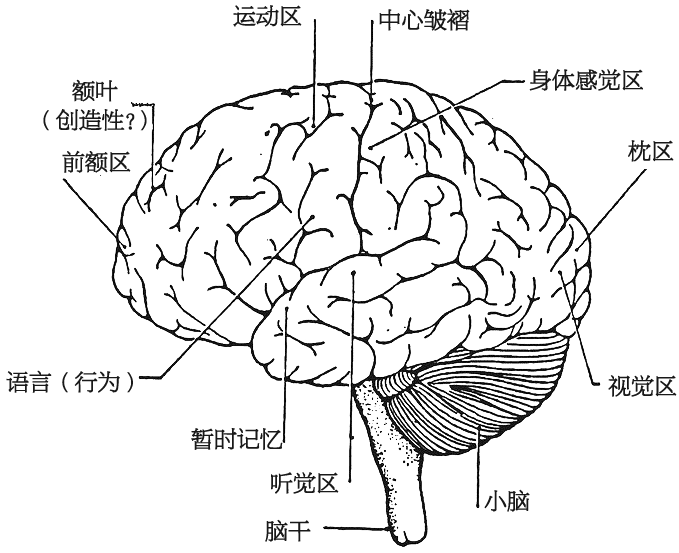
\includegraphics{img_066.png}
\caption[人脑左视阁。]
  {人脑左视图。奇怪的是视觉区在头的后部。[摘自史蒂文·罗斯的《有意识的大脑》,修订本,第50页。] }
\end{figure}

人脑从解剖学的角度看可以分成若干彼此相区别的部分,如大脑、小脑和下丘脑(见\fig{66})。大脑是人脑中最大的部分,它可分成左半球和右半球。每个半球的外面几毫米被分层的“壳”包裹着,这就是大脑皮层。从解剖学上看,大脑皮层的总量是人脑区别于低智能物种的脑的重要特征。我们不准备详细描述大脑的任何子器官,因为迄今为止在这些大尺度子器官和它们所负责的心智或物理活动之间只能建立起最粗略的对应。例如,已经知道语言主要是由两个半球之一来掌握的——事实上通常是左半球。我们还知道小脑的作用是发送一系列脉冲到肌肉,以控制运动。但是,这些区域是如何完成它们的功能的,这在很大程度上还是个谜。

\section{脑之间的映射}

说到这里,一个极其重要的问题出现了。如果思维的确是在脑中发生的,那么两个脑是如何彼此相区别的呢?我的脑和你的脑有什么不同呢?你的思想当然和我的不会完全一样,对其他任何人来说也如此。但我们的大脑都具有相同的解剖学划分。脑之间的这种一致性可以扩展到什么程度?能达到神经元层次上吗?如果你观察那些在思维的层次体系中处于足够低的位置上的动物——例如低等的蚯蚓,答案将是肯定的。下面的引文摘自神经生理学家大卫·休贝尔在一次会议上的讲话,这次会议的议题是与地球外的智能生物通讯。

\begin{quote}
我估计像蚯蚓这样的动物会拥有数以千计的神经细胞。非常有趣的是,我们可以在一条特定的蚯蚓身上标出一个特定的单个细胞,然后在同一品种的另一条蚯蚓身上找到一个与之相对应的细胞。\note{卡尔·萨根[Carl Sagan](编),《与天外智能通讯》[\bn{Communication with Extraterrestrial Intelligence}],第78页。}
\end{quote}
蚯蚓具有同构的脑,人们甚至可以说,“只存在一条蚯蚓。”

但是,随着你观察的对象在思维层次体系中的上升及其神经元个数的增加,这种不同个体的脑之间的一一映射关系很快就消失了——这支持了你的猜疑:不是只存在一个人!然而,一旦在比单个神经元大、又比脑的主要子器官小的尺度上把不同人的脑相比较,仍然可以发现显著的物理相似性。个体的精神差异是如何表现在脑的物理结构上的?上述事实对这个问题来说意味着什么?如果我们来观察我的神经元的相互联系,我们是否能发现各种结构,它们可以被确定为以编码的形式表示了我所知道的特殊事物、我所具有的特殊信念、我怀有的特殊愿望、恐惧和好恶?如果精神体验可以归因于大脑,那么知识和精神生活的其它方面是否也能类似地追溯到大脑中的特定位置,或大脑特定的物理子系统?这是我们在本章和下一章中要不断涉及的一个中心问题。

\section{大脑过程的定位:一个谜}

为了回答这个问题,神经病学家卡尔·拉施利从1920年左右开始进行了多年实验,试图发现老鼠在脑中的哪个地方存贮了它跑迷津的知识。史蒂文·罗斯在他的著作《有意识的大脑》中这样描述了拉施利的尝试与磨难:

\begin{quote}
拉施利试图确定记忆在皮层中的位置,为此,他首先训练老鼠跑迷津,然后切除皮层的不同区域。他让动物进行恢复,然后检查跑迷津技能的保持情况。出乎他意料的是,要找到一个迷津通路的记忆能力所对应的特定区域是不可能的。相反,所有进行了皮层局部切除的老鼠都受到某种损害,而损害的程度大致正比于皮层的切除量。皮层切除破坏了动物的运动和感觉能力,它们可能一瘸一拐,步态蹒跚,但总能设法穿过迷津。就记忆而论,皮层似乎是等势的,这就是说,所有的区域都有相同的可能效用。后来,在他发表于1950年的最后一篇论文“寻找记忆痕迹”中,拉施利沮丧地断定唯一的结论是记忆根本就是不可能的。\note{史蒂文·罗斯,《有意识的大脑》,第251--252页。}
\end{quote}

奇妙的是,在40年代末,几乎在拉施利进行他的最后的工作的同时,支持相反观点的证据在加拿大出现了。神经外科医生怀尔德·潘菲尔德那时正在检查进行了某种大脑手术后的患者的反应。这种手术是把电极插入患者被暴露了的大脑的各种部位中,然后用微弱的电脉冲刺激那些与电极相接触的神经元或神经元群。这些脉冲和来自其它神经元的脉冲很相似。潘菲尔德发现:对某些神经元的刺激会可靠地给患者带来特定的幻像和幻觉。这些人工诱发的感觉是各式各样的,从陌生而不可名状的恐惧感到嗡嗡声及颜色等等不一而足。最令人印象深刻的是,其中还包括早年生活中事件的完整过程,比如童年时代的一次生日晚会。能触发这种特定事件的位置只限于一个很小的区域——基本上集中于一个单个神经元。于是潘菲尔德的这些结果戏剧性地回击了拉施利的结论:说到底,这些结果似乎意味着特定的记忆是由局部区域负责的。

对此我们该怎样理解呢?一种可能的解释是:记忆是局部编码的,但这种局部编码在皮层的不同区域反反复复地进行着——这可能是进化中发展起来的防卫策略,用来对付在战斗中或在神经生理学家所进行的实验中可能出现的皮层损失。另一种解释是:记忆可以从分布于整个大脑的动态过程之中重建,但可以从局部点触发。这一理论是基于现代电话网络的观念之上的,在这种网络中,一个长途呼叫的传送途径无法事先预料,因为这是在呼叫发出时才选定的,取决于整个电话网的状况。毁坏网络的任何局部都不会阻塞呼叫,而仅仅使它们在传送时绕开损坏的地区。在这个意义下,任何呼叫都潜在地是不可定位的。然而,任何呼叫都恰好联结了两个特定的点,在这个意义下,任何呼叫都是可定位的。

\section{视觉处理的特性}

一些有关大脑过程定位的最有趣、最有意义的研究工作,是在近十五年内由大卫·休贝尔和托斯坦·威瑟尔在哈佛完成的。他们绘出了猫脑中的视觉通道,它起自视网膜中的神经元,沿它们那些导向头部后方的路径通过侧膝体的“中继站”,终止于大脑正后部的视觉皮层。首先,由于有拉施利的结果,存在有界说良好的神经通道这一点是不同寻常的。但更不同寻常的是位于通道不同阶段上的神经元的性质。

已经发现,视网膜神经元基本上是对比感觉器。更具体地说,它们的活动方式是这样的:每个视网膜神经元通常都以一个“常规速率”发射。当视网膜上它所在的部分被光照射时,它的发射速率或是加快或是减慢,甚至可能停止发射。但是,它这样做的条件是视网膜的周围部分受到的光照较少。这意味着存在两种神经元:“开中心”和“关中心”。开中心神经元的特征是:在它们敏感的圆形视网膜区域中,当中心亮外围暗时,它们的发射率会上升;关中心神经元的特征是:当中心暗外围亮时,它们发射得快一些。如果把一个开中心模式显示给一个关中心神经元,它的发射率会下降(反之亦然)。均匀的光照将不影响这两种视网膜神经元,它们仍继续以常规速率发射。

从视网膜开始,信号从这些神经元出发,通过视神经到达接近大脑中部的侧膝体。在那里,我们可以发现视网膜表面的一个直接映像。之所以这样说,是因为侧膝体神经元只能被落在视网膜特定区域的特定刺激所触发。在这个意义下,侧膝体消失了,它似乎仅仅是一个“中继站”,而非进一步的处理器,(虽然公平地说,对比敏感性在侧膝体中有所增强)。视网膜图像按照侧膝体中神经元的发射模式以一种直接的方式编码,虽然事实上那些神经元不像视网膜那样分布于一个二维平面上,而是分布在一个三维团块中。这就既保持了信息又把二维映射到三维,形成了一个同构。表示方式维数的变化可能还有更进一步的意义,这一点还没有充分揭示出来。不管怎么说,尚未得到解释的视觉阶段实在太多了,以致于对下列事实我们不应失望而应高兴——在某种意义上,我们已经把这一个阶段弄清楚了!

\begin{figure}
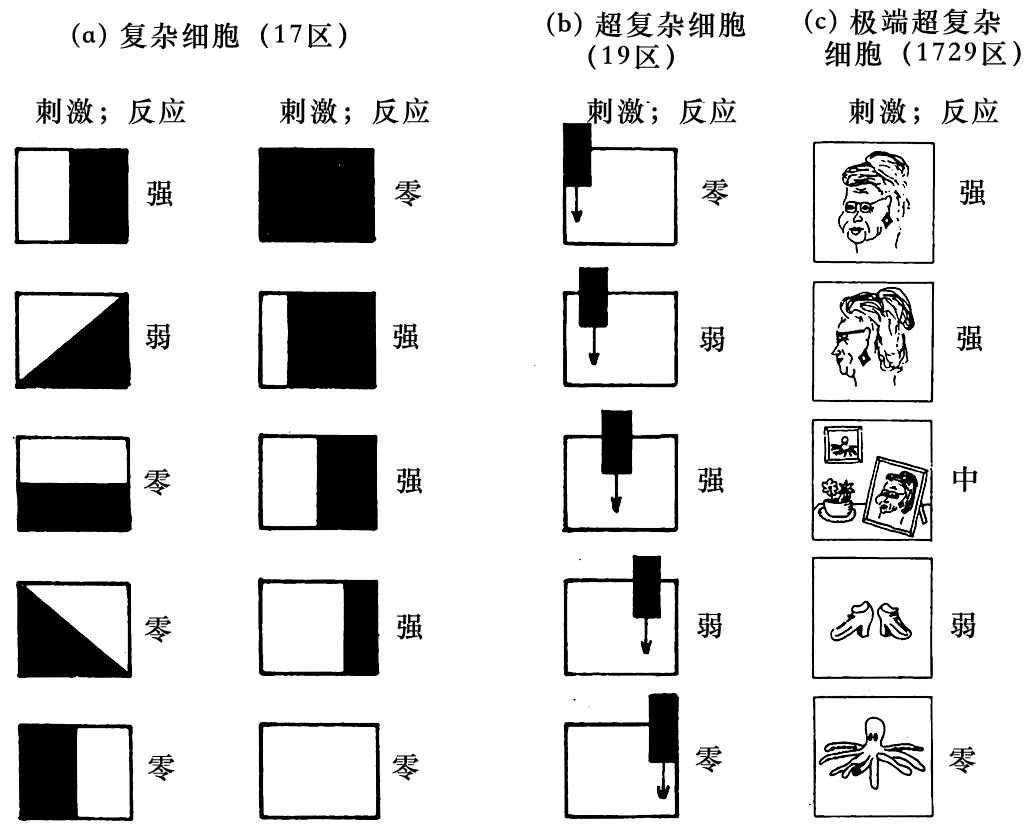
\includegraphics{img_067.png}
\caption[某些神经元样本对模式的反应。]
  {某些神经原样本对模式的反应。(a)这个负责边缘检测的神经原寻找左明右暗的垂直边缘。第一列显示了边缘的倾角与该神经原的关系,第二列说明边缘在域中的位置与这个特定神经原无关。(b)显示了超复杂细胞的更具选择性的反应:在这里仅当下行的舌状物通过域中间时反应最强。(c)假想的“祖母细胞”对各种随机刺激的反应。读者不妨思考一下对同一组刺激一个“章鱼细胞”将作何反应。}
\end{figure}

从侧膝体出发,信号向后传至视觉皮层。在这里某些新的加工出现了。视觉皮层细胞分为三类:简单的、复杂的和超复杂的。简单细胞的活动方式和视网膜细胞或侧膝体细胞相似:它们对视网膜特定区域中与背景形成对比的亮点或暗点作出反应。而复杂细胞则通常要从上百个其它细胞接收信息作为输入,识别视网膜上成特定倾角的明暗线条(见\fig{67})。超复杂细胞对应于沿特定方向运动的角、线条甚至于“舌状物”(也见\fig{67})。最后一种细胞是高度专门化的,因此它们有时被称为“高阶超复杂细胞”。

\section{一个“袓母细胞”?}

由于在视觉皮层中发现了能被复杂性不断增加的刺激所触发的细胞,有些人怀疑事情是否在向“一个细胞,一个概念”的方向发展——例如,你可能有一个“祖母细胞”,它当且仅当你的祖母进入视野时发射。这样一个“极端超复杂细胞”的多少带点幽默的例子不过是个玩笑,但是,可供选择的理论中哪个更合理,这并不是显而易见的。一种可能性是更大的神经网络被足够复杂的视觉刺激整体性地激活。当然,这些更大的多神经元单位的触发,可能以某种方式依赖于许多超复杂细胞发出的信号的整合。没人知道这是怎样完成的。正当我们似乎接近了“符号”怎样从“信号”中形成这一关键点时,线索中断了——一个吊人胃口的“且听下回分解”。但我们很快会回到这个故事,并努力再补充一些内容。

前面我提到过,人类的大脑之间在大的解剖学尺度上存在粗糙的同构,还提过蚯蚓的脑之间存在非常精密的神经元层次的同构。很有趣的是在猫、猴和人的视觉处理器官之间也有一个同构,其“粗细程度”介于粗糙和精密之间。这个同构是这样的:首先,三个物种都在脑的后部为视觉加工“特供”了一部分皮层,即视觉皮层。其次,在三者之中视觉皮层都分成三个子区域,称为皮层的17、18和19区域。这些区域仍具有普遍性,这就是说在三个物种的任何正常个体的脑中都可找到它们的位置。在每个区域中还可以再细分,一直到视觉皮层的“柱状”组织。柱状组织垂直于皮层表面,沿半径方向伸向内脑,其中绝大多数的视觉神经元间的联系是沿脑半径方向,即柱体的方向,而非建立于柱体之间。每个柱体映射到一小块特定的视网膜区域上。柱体的数目在不同的个体中是不同的,因此不可能找到“同一个柱体”。最后,在柱体内部,某些层主要由简单神经元构成,而另一些层主要由复杂神经元构成。(超复杂神经元往往在区域18和19中占数量优势,而简单和复杂神经元主要出现于区域17中)。看起来我们的分析细到这个程度就不会再有同构了。从这里直到单个神经元层次,每个猫、猴或人都有完全唯一的模式——有点像指纹和签名一样。

在猫脑和猴脑中的视觉加工之间,存在一个虽然次要但或许能说明问题的差别,这与把来自两眼的信息整合成单一的复合高层信号的时刻有关。研究结果表明,在猴脑中这一整合发生的时刻稍迟于猫脑,致使每个单眼信号都有稍长的独立加工时间。这并不值得惊讶,因为可以设想,一个物种在智能层次体系中所处的位置越高,其视觉系统所要处理的问题就越复杂,因此信号在最终得到一个“标签”前所要经过的预处理也就越来越多。对初生牛犊视觉能力的考察已经非常戏剧性地证实了这一点。小牛似乎一生下来就已经达到它将来所可能具有的视觉分辨力。它会胆怯地回避人或狗,但不怕别的牛。有可能它的整个视觉系统在出生前就被“硬性联接”了,而且只涉及较少的视觉皮层。与此相反,人的视觉系统深深地依赖于皮层,而且要经过若干年才能成熟。

\section{汇集到神经模块}

令人迷惑不解的是,在迄今为止关于脑组织的发现之中,并没有找到多少大尺度硬件和高层次软件之间的直接对应关系。举例来说,视觉皮层就是块大尺度硬件,它的软件用途是很清楚的——视觉信息加工,但至今发现的所有加工过程仍都是层次很低的,远没有接近对象识别在皮层中的定位。这意味着没有人知道复杂细胞和超复杂细胞的输出在哪里或怎样转换成对形状、位置、图像、面容等等有意识的识别。人们已在寻找证据,试图证明许多低层次的神经反应“汇集”成越来越少的高层反应,最终达到像所谓的祖母细胞一类的东西,或是前面提到过的某种神经元网络。显而易见,这个发现不会出于某种粗略的解剖学划分,而是需要进一步的微观分析。

替代祖母细胞的一种可能解释是,在这一“汇集”过程的终点处有一组神经元,比如说有数十个,当祖母进入视野后它们全都发射。对于每个不同的可识别的对象,都有唯一的一个神经元网络和一个“聚焦”于该网络的汇集过程。沿着类似的思路还可以提出更复杂的解释,包括可以用不同的方式而非固定方式激活的网络。这样的网络就是我们大脑中的“符号”。

但这种“汇集”是必须的吗?或许一个被辨认的物体就是以它在视觉皮层上的“印迹”来隐含地标识的——所谓“印迹”,是指来自简单、复杂和超复杂细胞的集体反应。或许大脑并不需要什么进一步的识别机制来识别一个特定形状。但是,这种理论将造成一系列问题。假设你在欣赏风景,这在你的视觉皮层上留下了印迹,但此后你怎样才能从中得到关于这个景象的词语描述呢?举例来说,法国后印象派画家爱德华·维亚尔的作品,往往需要几秒钟的审视,然后一个人的形象才突然呈现在你面前。大概只须片刻其印迹就能形成于视觉皮层上——但这幅画是在几秒钟后才被理解的。这只是一个例子,实际上这种现象很普遍——在识别时好像感到有什么东西在你的脑海里“结晶”了,这一过程不是发生在光线射在你视网膜上的时候,而是稍迟一些,要等到你智力的某些部分有机会作用于视网膜信号之后才行。

“结晶”这个比喻从统计力学的角度提供了一幅恰当的图像。在这个图像里,介质中的无数微观的互不相干的活动缓慢地造成局部区域的内在一致性,这一区域不断扩展,最终这无数微观事件会对其介质产生根本性的结构改造,使其从一个杂乱无章彼此独立的元素集合体,变为一个大的、一致的、内在联系紧密的结构。如果你把早期神经元活动看作独立的,而把它们这许多独立发射的最终结果看作是触发了一个界说良好的大神经元“模块”,那么“结晶”这个词似乎再贴切不过了。

汇集过程的另一个论据基于如下事实:使你感到你看见了同一个对象的景象可以有无数多个——例如你的祖母,她可能喜也可能愁,可能戴帽子也可能没戴,可能在明亮的花园里也可能在昏暗的车站中,可能近也可能远,可能侧对着你也可能面向着你,如此等等。这些场景会在视觉皮层上产生极其不同的印迹,但它们都能使你叫“喂,奶奶”。因此,一个汇集过程必定出现于接收到视觉印迹后,但又在词语发出前的某一时刻。有人可能主张这种汇集不是对祖母的感知的一部分,而仅仅是词语表达过程的一部分。但把过程做这样的划分看上去很不自然,原因是你可以在内部使用“这是奶奶”这一信息,同时又没有任何词语表达。当然,在整个视觉皮层上处理全部这些信息未免太笨拙了,实际上其中大部分都该扔掉,因为你根本不关心影子落在哪里或她罩衫上有多少扣子这类事情。

如果在理论上不承认存在有汇集过程,那么另一个困难是需要说明为什么对同一个印迹会有不同的解释——例如艾舍尔的画《凸与凹》(\fig{23})。正如这样一个显而易见的事实;我们从电视屏幕上感知到的不仅仅是点,还有组块,而且,假定当一片点状印迹产生于视觉皮层上之后感知就已经发生,这似乎有些荒唐。一定是有某种汇集,其最终效果是触发某些特定的神经元模块,而每个模块都关联于场景中的概念——或称组块。

\section{作为思维过程媒介的模块}

于是我们可以作出这样的结论:对应于每个概念,都存在一个界说良好的可触发模块——由一小群神经元构成的模块——也就是前面设想过的那种“神经复合体”。这个理论有个问题——至少朴素地看是如此——它使人想到应该能够在大脑里确定这些模块的位置。迄今为止还没有做到这一点,而且存在一些反对定位化的证据,如拉施利的实验。但是,现在下结论未免为时过早。每个模块都可能有多个复本分布在各处,也可能模块在物理上相互重叠,这两种效应都倾向于使把神经元分成“包裹”的界限变得模糊不清。或许复合体像摞成一摞的纸张,偶尔会互相交叉;或许它们像互相缠绕的长蛇,在这里或那里像眼镜蛇的头那样伸出来;或许它们像蜘蛛网;或许它们是某种电路,信号在里面转来转去,比扑向蚊虫的燕子还难以捉摸。到底是什么谁也不知道。这些模块甚至可能是软件现象,而非硬件现象——这一点我们过一会儿再讨论。

这些假设性的神经元复合体可以使人想到许多问题,例如:
\begin{enumerate}
\item 它们是否延伸到了脑的内部区域,如中脑和下丘脑等处?
\item 单独的一个神经元能否属于一个以上这种复合体?
\item 单独一个神经元可以属于多少个这种复合体?
\item 一个这种复合体可覆盖多少神经元?
\item 对每个人来说,这些复合体是否大致相同?
\item 在不同的人脑中,是否能在对应的位置找到对应的复合体?它们在每个人脑中的覆盖方式是否相同?
\end{enumerate}

从哲学上看,所有这些问题中最重要的是:这些模块——例如一个祖母模块——的存在说明了什么?这是否使我们对自身的意识现象有所认识?还是说这和仅仅知道“大脑是由神经元和胶质细胞所组成”一样,仍使我们对意识是什么一无所知?也许你在读《蚂蚁赋格》时已经猜到,我的感觉是,要想理解意识现象,我们还得经过一个漫长的过程。需要完成的关键步骤是:对同一个脑的同一个状态来说,低层次的描述——面向神经元的——要变成高层次的描述——面向模块的。或者再一次重申《蚂蚁赋格》中带有启发性的术语,我们需要的是把脑状态的描述从信号层转向符号层。

\section{活跃的符号}

让我们从现在开始把这些假设性的神经复合体、神经模块、神经包、神经网络、多神经元单元——你可以随便叫它们什么,也不管它们的形状是一摞纸、园艺耙还是眼镜蛇、小雪花——统称作“符号”。用符号的说法来描述大脑状态,这在对话中已经提到过了。这样一个描述会是什么样的呢?把什么样的概念设想成为“符号化”了的才算是合理的?符号之间会有什么样的相互关系?这幅图景又为对意识的认识提供了什么见解呢?

首先要强调的是,符号既可能是休眠的,也可能是觉醒的(激活的)。活跃的符号就是那些已经被触发了的——即其中由外部刺激造成发射的神经元数目已经达到了阈值。由于一个符号可以通过许多不同方式来触发,因此它在觉醒状态下可以按许多不同的方式活动。这提示我们不应把符号看成一个固定的实体,而应看成一个可变的实体。因此,仅仅通过说“符号A、B、C……N是所有活跃符号”来描述大脑的一个状态是不够的,我们还必须为每个活跃符号提供一组附加参数,以刻划该符号内部工作的某些方面。一个有趣的问题是,在每个符号中是否都有某些核心神经元,它们在符号被激活时一定是发射的?如果这样一个神经元核心团存在,我们可以称之为该符号的“恒定核心”。作下面这样的假设是很诱人的:每当你想到一个事物,例如瀑布,某种固定的神经过程就重复进行,这些过程无疑在细节上依当时的情景会有不同,但总是可靠地发生。不过,是否果真如此还不清楚。

那么一个符号在觉醒时做些什么呢?一个低层次的描述可能是:“它的许多神经元发射了”。但我们已经对此不感兴趣了。高层次的描述应消除一切涉及神经元的说法,而完全集中于符号。这样,一个关于符号如何是处于活跃状态而非休眠状态的高层次描述就会是“它发出消息——或称信号——其目的是试图唤醒——或触发——其它符号”。当然这些消息是被神经元以神经脉冲流的方式承载的——但我们应尽可能避免使用这种表达方式,因为这代表着一种低层次的观察事物方法,而我们希望能完全在高层次上进行描述。换句话说,我们希望思维过程可以被设想成与神经事件相隔离,正好像一座钟的行为可以与量子力学定律相隔离,或细胞生物学可以和关于夸克的定律相隔离一样。

但这样一幅高层次的图景有什么好处呢?为什么“符号A和B触发了符号C”比“神经元183通过612刺激了神经元25并导致了它的发射”要好一些?在《蚂蚁赋格》中回答了这个问题:这是因为符号把事物符号化了,而神经元不是如此。符号是概念的硬件实现。一组神经元触发另一个神经元并不对应于外部事件,而一些符号对某个符号的触发却以某种方式对应着现实世界——或某个假想世界——中的事件。符号间通过来回传送消息来保持联系,其方式使得符号的触发模式与在我们的世界中发生的——或在一个类似于我们的世界中可能发生的——大尺度事件十分相像。意义在这里出现的原因实质上恰如在pq系统中的情形一样——同构。只不过在这里这个同构已变得极其复杂、微妙、精巧、多面化,而且是内涵的。

而且,符号能够来回传递复杂的消息,这一点就足以使得神经元自身无法充当符号的角色。因为神经元仅用唯一的方式发送信息,不能带有选择性地使一个信号一会儿发往一个方向,一会儿又发往另一个方向,所以它完全不具有选择性触发能力,而这种能力是符号在模拟现实世界中的对象时所必须具有的。威尔逊在他的著作《昆虫社会》中,指出了蚁群内部消息传播的类似特点:

\begin{quote}
\lnote{(大众传播)}可定义为在群体中并非以一个个体传向另一个个体的方式所进行的信息传递。\note{爱德华·威尔逊,《昆虫社会》,第226页。}
\end{quote}
看来把大脑想象成一个蚁群并不算太荒唐!

下一个问题——这也是一个极端重要的问题——与大脑中单个符号所代表的概念的性质和“尺寸”有关。关于符号的性质存在这样一些问题:到底是存在一个代表瀑布的一般观念的符号,还是各个具体的瀑布对应于不同的符号?或者上述两种方案同时都实现?关于符号的“尺寸”存在这样一些问题:是否存在一个代表一个完整的故事、一段旋律、或一个笑活的符号?或者,作为更大的可能,符号只相应于像词这种规模的概念,而更大尺度的,如短语和句子,可以表示成不同符号的同时或顺序的激活?

让我们考虑一下符号所表示的概念的规模这一问题。大部分表达成句子的思想都是由一些基本的、像原子似的成分所构成,而对这些成分我们一般是不作进一步的分析的。这大致就是词的规模——有时长些,有时短些。例如,名词“瀑布”、专有名词“尼亚加拉瀑布”、表示完成的虚词“了”、动词“赶上”以及更长的固定短语都是接近于原子化的。这都是一些典型的基本笔触,我们就是用它们来绘出更复杂概念的肖像,例如一部电影的情节、一座城市的风情、意识的性质等等。这些复杂的概念都不是单一的笔触。认为语言的笔触也就是思维的笔触,这看起来是合理的。因而符号所表示的概念大概也就是这种规模的。这样,一个符号大略对应于那些你可用一个词或一个固定短语所表示的东西,或者对应于那些你指定了一个专有名称的东西。而在大脑中表示更复杂的观念——例如恋爱中碰到的一个难题——则可能需要一个非常复杂的符号激活序列。

\section{类与例}

在思维中有一种一般性的区别:范畴与个体,或类与例(另外两个有时会用到的词是“型”与“例”)。初看起来似乎一个给定符号应当固有地或者是一个类符号,或者是一个例符号,但这么想是过于简单化了。实际上,大多数符号可以扮演二者中任何一个角色,这取决于它们的激活环境。例如下列序列:

\hangparshape{10}%
(1)\enspace 一种出版物\\
(2)\enspace 一种报纸\\
(3)\enspace 《中国日报》\\
(4)\enspace 五月十八日的《中国日报》\\
(5)\enspace 我的那份五月十八日《中国日报》\\
(6)\enspace 我的那份五月十八日《中国日报》,在我第一次拿起它的时候(而不是几天后在我的炉子中燃烧时)

在这里,第二行到第五行都扮演着双重角色。其中,第四行是第三行对应的一般类的一个例,而第五行又是第四行的一个例。第六行是一个类的一种特殊例:一个“表现”。一个对象在其生存历史中相继所处的阶段是它的各个表现。有趣的是,不知道一个农庄中的母牛是否能感知到,在那个喂它们干草的快活农民的所有表现的背后有一个不变的个体。

\section{原型原则}

看起来,上面那个序列是关于一般性的一个层次结构。其顶层是一个非常一般的概念范畴,底层是某种在确定的时空位置上的低级的特定事物。但是,如果认为一个“类”必定总是非常一般和抽象的,这就未免局限性太大了。其原因是我们的思维采用了一种机智的原则,我们可以称其为“原型原则”:

\begin{block}
最具体的事件可以被用作一类事件的一个一般范例。
\end{block}
我们都知道,特殊事件具有一种生动性,这使得它们可以被牢牢印在记忆中,以便后来被当作在某个方面与它们相似的其它事物的模型。因此,在每个具体事件中,都蕴含着全部相似事件组成的类的萌芽。一般性即寓于特殊性之中,这个思想具有深远的重要性。

至此我们自然会问:大脑中的符号是表示类,还是表示例?是否某些符号只表示类,而另一些符号只表示例?或者说一个符号可以交替完成类符号和例符号双重职责,这取决于它的哪一部分被激活?后一种理论看起来很有吸引力,有人可能会设想一个符号的“轻微的”激活可能代表一个类,而更深入的,或更复杂的激活可能包括更细致的内部神经发射模式,因而是表示一个例。但再一想,这样太古怪了。比如,这意味着如果以足够复杂的方式激活代表“出版物”的符号,你就能得到一个非常复杂的符号,它代表着在我的炉子中燃烧的一份特定的报纸。而且所有其它印刷品的所有其它可能的特例均可通过对代表“出版物”的这个符号的某种方式的激活来内在地表示。对“出版物”这个符号来说,这样一副担子似乎太重了。因此我们只能下结论说:例符号可能和类符号同时存在,而不仅仅是后者的激活方式。

\section{从类中分离例}

另一方面,例符号的许多性质常常是从它所隶属的类中继承来的。假设我告诉你我去看了个电影,你将开始“铸造”那个特定电影的一个新的例符号。但在缺乏更多信息的情况下,这个新的例符号不得不紧密地有赖于你关于“电影”的已有的类符号。你将不自觉地依靠许多关于该电影的预先假定——例如,它的放映时间在一小时至三小时之间,是在本地一家剧场上映的,内容是关于某些人的一个故事,等等。这些都作为与其它符号的可能联系(即潜在的触发关系)而被构造在类符号中,称为“缺席选择”。在任何新铸造的例符号中,缺席选择都可以很容易地被取消,但如果没有明确地这样做,它们就会被例符号从类符号中继承并保留下来。它们将采用“规范型”(或者说类符号)所提供的一些合理猜测为你对这个新的例——例如我所看的电影——的考虑提供一些初步的根据,直到它们被取消为止。

这就像一个既无主见也没经验的孩子——他完全依赖于父母的经验和见解,只会鹦鹉学舌。但渐渐地,随着与世界的其它部分的相互作用不断增多,这个孩子获得了他自己的独特经验,并不可避免地会离开父母。最后,孩子羽翼丰满,成了大人。一个新的例也能以同样的方式通过一段时间从它的“父母”类中分离出来,凭本身的资格成为一个类或一个原型。

为了形象化地描述这种分离过程,假设在某个周末的下午你打开了收音机,碰巧收听到两个“随机的”球队之间的一场橄榄球赛。开始你不知道其中任何一个队员的名字。此时解说员说道:“回文斯接住球以后,就一直往前,达阵得分了!”这时你所记住的只不过是某个队员接到了另一个队员的球,并达阵得分了。因此这种情况是类符号“橄榄球队员”被激活,同时以某种方式被并行激活的还有关于带球的符号。但后来回文斯又出现在一些关键的时刻,你开始专门为他建立一个新的例符号,或许以他的名字为中心。这个符号像个孩子似地依赖于类符号“橄榄球队员”:你关于回文斯的大部分想象都来自于你在符号“橄榄球队员”中存放的关于橄榄球队员的规范型。但渐渐地,随着你得到的信息的增多,“回文斯”这个符号变得越来越具有自主性,对需要并发激活其父母类符号的依赖性逐渐减少。只要回文斯做出一些精彩的动作,表现出众,上述过程可能仅在几分钟内就发生。但他的队友们仍可能全由类符号的激活所代表。最后,可能在几天之后,你在报刊的体育专栏中读到了某些文章,这时“脐带”断了,回文斯可以独立存在了。至此你知道了他的故乡、他的爱好等情况,你记住了他的相貌,如此等等。到了这时,回文斯不再仅仅被认作是一个橄榄球运动员,而是首先是一个人,他正好也是个橄榄球队员。“回文斯”这个例符号于是可以在其父母类符号(橄榄球队员)处于休眠状态时被激活了。

回文斯这个符号一度是围绕其父母符号运转的一颗卫星,正像一颗绕地球转的人造卫星一样,只是后者要大得多也重得多。然后进入一个中间阶段,此时虽然一个符号比另一个重要,但它们可以被看成是互相围绕的——有点像地球和月亮。最后,新符号变得非常自主了,此时它可以很容易地成为类符号,并开始有新的卫星绕着它转——一些相应于其它人的符号,他们还不为你所熟悉,但和回文斯有某些共同之处,因此你可用回文斯作为他们的临时规范型。等到你获得更多的信息后,这些新符号也随后都具有自主性了。

\section{搞清符号间的纠葛是很难的}

一个例在类中的生长以至最终脱离所经过的各个阶段,可以通过有关符号的联接方式的不同来区分。毫无疑问,有些时候很难分清在何处一个符号终止而另一个开始。一个符号怎样才算比另一个符号“更为活跃”?如果一个符号的激活可以独于另一个符号,那么称它们为自主的将是很明智的。

我们在前面用到了一个天文学的比喻。有趣的是,行星的运动是一个很复杂的问题——事实上,尽管进行了几个世纪的工作,三个天体通过万有引力相互作用(例如地球、月亮和太阳)的一般问题还远没有得到解决。但在下述情形之下,有可能得到一个良好的近似解:其中一个天体的质量远比另外两个大(在这里是太阳)。此时可以把这个天体看作静止的,另外两个天体围绕它转动,最后再加上两个卫星间的相互作用。但这种近似要求先把系统分解成太阳和一个“簇”:地球—月亮系统。这是一个近似,但能使我们对该系统有很深入的理解。这样,这个簇在多大程度上是现实的一部分,在多大程度上是人脑所臆造的,是人强加给宇宙的一种结构呢?这种在感知到的自主或半自主的簇之间所划的界限的“现实性”问题,当联系于大脑中的符号时,会带来无穷无尽的麻烦。

一个非常令人迷惑的问题是“名词复数”这样一个简单的问题。比如说,我们是怎样形成一个茶杯中有三只鸡,或一个电梯里有几个人的图像的?我们是不是从“鸡”的类符号开始,然后从它上面抹下三个“复本”?也就是说,我们是不是用类符号“鸡”作模板,构造了三个新的例符号?还是连带地激活符号“三”和“鸡”?如果往这些想象的场景中或多或少地添加些细节,那上述两种说法都会变得难于站住脚。例如,我们显然不是为所见到过的每个鼻子、胡子、盐粒等等都分别设立例符号。我们用类符号来处理这些为数众多的项目,因而当在街上遇到留胡子的人时,我们仅仅以某种方式激活类符号“胡子”,而不是铸造新的例符号,除非我们观察得很仔细。

另一方面,一旦我们开始区分不同的个体,就不能再依赖于用一个类符号(如“人”),以分时的方式来处理全部不同的人。很清楚,对于个别的人必须设置不同的例符号。若是想靠玩“杂耍”来完成这一任务——就是说,靠一个类符号在若干种不同的激活方式(每种分别对应于某个人)之间飞来飞去——那是很荒谬的。

在这两种极端情况之间,一定存在着许多种中间情况。很可能在大脑中有多种方式进行类与例的区分,从而产生具有不同程度的特殊性的符号及符号组织,而这些方式形成一个完整的层次结构。下列不同种类的个体和符号的连带激活可能会造成具有各种程度特殊性的心理映像:

\begin{enumerate}
\item 单个类符号的各种不同激活方式或深度;
\item 若干个类符号以某种并行方式同时激活;
\item 激活单个例符号;
\item 在激活单个例符号的同时激活若干个类符号;
\item 以某种并行方式同时激活若干个例符号和若干个类符号。
\end{enumerate}

这又把我们带回到一个老问题:“一个符号何时才能成为脑的一个可辨别的子系统?”例如,考虑上面第2种情况:若干个类符号以某种并行方式同时激活。在所考虑的概念是“钢琴奏鸣曲”时,上述情况很容易发生(至少相应于“钢琴”和“奏鸣曲”的两个符号正被激活)。但如果这对符号连带激活的次数足够多,则有理由假设它们之间的联系会变得很强,致使它们在以适当方式被共同激活时,将像一个单元一样活动。因此,在适当的条件下,两个或更多的符号能像一个符号一样活动,这意味着数出大脑中符号的数目要比预想的更困难。

有时会出现这样的情况:两个以前互不相关的符号以一种并行方式同时被激活。它们可能联系得很紧密,似乎是一个必然的共同体,而且两个老符号的强相互作用形成了一个独立的新符号。如果上述情况出现了,对新符号怎样说才好呢?是说“它一直存在但从未被激活”,还是说它已经被“制造”出来了?

如果说这听起来太抽象,让我们举一个具体例子:对话《螃蟹卡农》。在对话的创作过程中,两个已有符号——一个代表“螃蟹卡农音乐”,另一个代表“言语对话”——被同时激发,并在外力作用下以某种方式产生了相互作用。一旦这种情况出现,后面的事情就是不可避免的了:一个新符号——是个类符号——从二者的相互作用中产生,并从此能被独立激活。那么它是否本来就是我大脑中的一个休眠符号?如果是这样,那它一定也是任何人大脑中的休眠符号,只要他具有作为其成分的符号,哪怕它从未被从那些作为成分的符号中唤醒过。这就意味着要数出任何人大脑中的符号,就必须包括全部休眠符号——即全部已知符号的全部激活类型的全部可能的排列组合。这甚至应包括睡觉时大脑创造的那些稀奇古怪的软件产物——那些在它们的主人进入梦乡时被唤起的奇特的观念混合物……这些“潜在符号”的存在表明,把大脑想象成一个处于界说良好的激活状态的界说良好的符号集合,的确过于简单化了。而在符号层次上准确刻划大脑的状态则要远远困难得多。

\section{符号——是软件还是硬件?}

由于在每个人的大脑中都存放着数量众多甚至仍在不断增加的符号,你可能会问是否有一天大脑终于会饱和——那时新符号将不再有容身之处。推测起来,这种情况的出现条件是符号不彼此重叠。——如果一个给定的神经元从不身兼二任,符号就会像电梯里的人一样。“注意:这个大脑的最大容量是$350275$个符号!”

但是,这并不是大脑功能的符号模型的一个必然性质。事实上,符号间的重叠和缠结很可能已成惯例,因此每个神经元也许会成为上百个符号的功能部件,而远不是只属于一个符号。这有点让人摸不着头脑了,因为如果真是这样,那不是很容易变成每个神经元都是任何符号的一部分了吗?若是如此,无论什么样的符号定位都不可能存在——每个符号都将对应于整个大脑。像拉施利的鼠脑皮层切除试验那样的结果可以因此而得到解释——但这同时意味着放弃我们开始时的想法,即把大脑分成具有不同性质的物理子系统。我们前面把符号刻划成“概念的硬件实现”就可能是个过于简单化的想法了。事实上,如果每个符号都是由和其它符号相同的神经元组成的,那说“不同的符号”还能有什么意义呢?什么是一个给定符号的激活特征?就是说,怎样才能把符号A的激活与符号B的激活区别开?我们的整套理论不就要付之东流了吗?而且即使不存在符号间的完全重合,符号之间实际重叠得越多,我们的理论不也就越难以维持吗?(\fig{68}显示了一种描绘符号重叠的可能方式。)

\begin{figure}
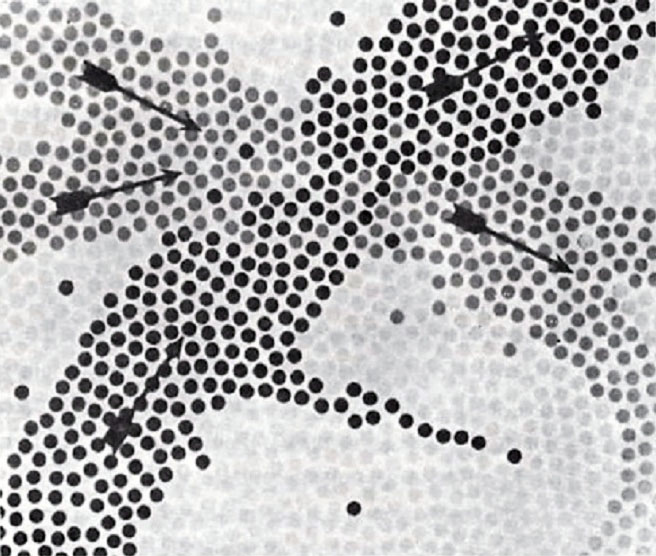
\includegraphics{img_068.jpg}
\caption[互相交叉的神经通道。]
  {在这张示意图中,假设神经原成点状分布在一个平面上。两条互相交叉的神经通道用不同的灰度来表示。可能出现这样的情况:两个独立的“神经闪电”同时通过这两条通道,像池塘水面上的两个涟漪一样彼此穿过(见\fig{52})。这形象地说明了两个共享神经原的“活跃符号”是如何可能同时被激活的。[摘自约翰·西·艾克勒斯[John C.Eccles],《面对现实》[Facing Reality],纽约:Springer Verlag,1970年版,第21页。] }
\end{figure}

有一种办法可以维护一个基于符号的理论,哪怕这些符号在物理上重叠得很厉害甚至完全重合。想一想一个池塘的水面,它可以承载许多不同的波浪和涟漪。硬件——即水自身——在所有情况下都是同样的,但它具有不同的可能激活方式。这样,同一个硬件的软件激活方式就都可以互相区别。使用这一类比时,我无意要走得那么远,以至于认为所有不同的符号只不过是在统一的神经介质上传播的不同类型的“波”,而这种介质不能以有意义的方式划分成物理上可区分的符号。但可能的情况是,为了把一个符号的激活与另一个符号的激活相区别,所完成的过程不仅要涉及发射神经元的定位,而且还需精确地确定那些神经元发射间的时间关系。这就是说,哪个神经元超前于哪些其它神经元?超前多少?一个特定神经元每秒发射多少次?这样或许若干符号可以共存于同一组神经元中,其中每个符号都有特征不同的神经发射模式。一种理论认为存在硬件上可区分的符号,另一种理论认为符号可以重叠,但能靠激活方式来彼此区别,这样两个理论的不同是前者给出的概念实现是硬件的,而后者给出的概念实现是部分硬件、部分软件的。

\section{智能的可抽取性}

为阐明大脑中发生的思维过程,我们还剩下两个基本问题。一个是解释低层次的神经发射通讯是如何导致高层次的符号激活通讯的,另一个是自足地解释高层次的符号激活通讯——建立一个不涉及低层神经事件的理论。如果后者是可能的——这是目前进行的所有人工智能研究的基础中的一个关键假设——那么智能就可能实现于不同于大脑的其它硬件上。那将表明智能是一种可以从它所在的硬件中“抽取”出来的性质——换句话说,智能将是一种软件性质。这将意味着意识和智能这一现象的确和大多数其它复杂的自然现象一样是高层次的:它们有自身的高层规律,这些规律依赖于低层,但又可以从低层中“抽取”出来。相反,如果没有全部由神经元(或模拟神经元)组成的硬件就绝对无法实现符号触发模式的话,这将意味着智能是一种局限于人脑的现象,比起那种可以用一个具有若干不同层次的规律体系来说明的现象,对它的解释要困难得多。

\begin{figure}
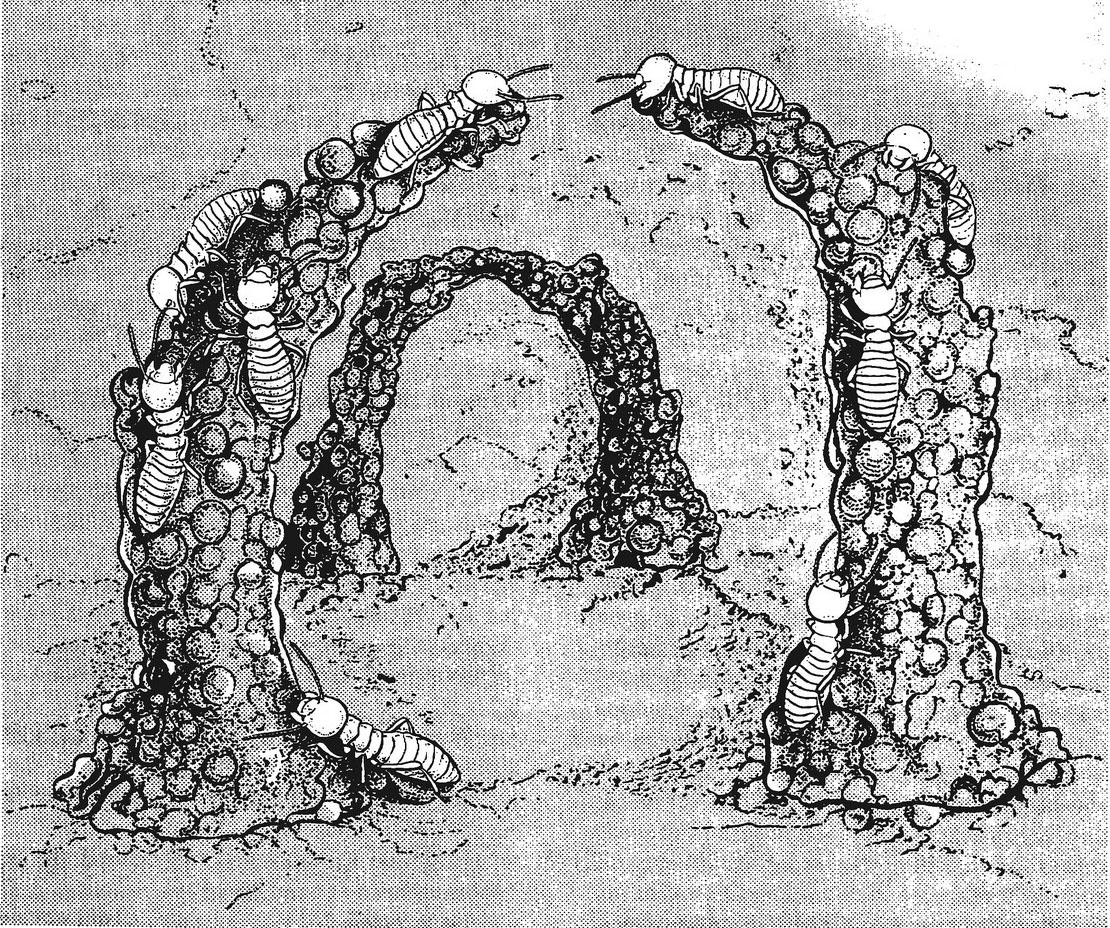
\includegraphics{img_069.jpg}
\caption[结队的工蚁在建一座拱。]
  {大白蚁中的工蚁在建一座拱。每颗杆子都是通过添加小团的泥土和排泄物来建立的。在左边柱子的顶端可以看到一个工蚁在安放一个圆粪团。其它工蚁正叨着小团往柱子上爬,并把它们放置在增长的一端。当柱子达到一定的高度时,白蚁们开始以一定的倾角使它向相邻的柱子的方向伸展,这显然是在气味的引导下进行的。在背景上可以看到一个完成了的拱。[图立德·何达布勒画,摘自成尔逊的《昆虫杜会》,第230页。] }
\end{figure}

这里我们要回到蚁群那神秘的集体行为。它们能建造巨大而复杂的蚁穴,尽管事实上一只蚂蚁的脑中仅有约十万个神经元,几乎不可能载有关于蚁穴结构的任何信息。那么蚁穴是如何构造的呢?信息来自何处?特别是可以考虑一下从哪里能找到描述一个\fig{69}所示的拱的信息。它们一定是以某种方式散布在蚁群中,在等级分布中,在年龄分布中——而且很可能大部分在蚂蚁身体内部的物理性质中。那就是说,蚂蚁间的相互作用被其脑中存贮的信息所左右的程度,差不多等同于被其下列特点所左右的程度:如它们有六条腿,它们的身体长度是多少多少,如此等等。有可能存在一个人工蚁群吗?

\section{单个符号能否被隔离出来?}

是否有可能在与所有其它符号相隔离的条件下唤醒一个符号?大概不行。正好像世界上的对象总是存在于其它对象组成的环境中一样,符号也总是联系于其它符号所组成的星云。这并不一定意味着符号不可能摆脱其它符号的纠缠。打一个简单的比方:雄性和雌性在一个物种中总是同时出现的,它们的作用是完全交织在一起的,但这并不是说雄雌没办法区分。每个对象都反映在其它对象中,正像因陀罗之网中的明珠彼此反映一样。在第五章中,函数$\mF(n)$和$\mM(n)$的交叉递归并不妨碍每个函数具有自己的特点。互相交织的F和M可以由一对互相调用的RTN反映出来。于是我们又可以转到由彼此交织的ATN组成的一个完整网络——一个由相互作用的递归过程组成的异层结构。在那里,缠绕是固有的,每个ATN都不能孤立地被激活,但它的激活又完全是可辨别的,不会与任何其它ATN相混淆。看来把大脑想象成一个ATN群并不算太荒唐!

类似地,相互之间存在多重联系的符号也是交织在一起,但又应当能彼此区分的。这可能涉及到识别神经网络,即一个网络及其激活方式——或者也可能是某种完全不同的东西。无论在何种情况下,如果符号是现实的一部分,那大概就能用一种自然的方式把它们在一个真实的大脑中描绘出来。但是,如果某些符号最终在大脑中被辨识出来,这也不意味着其中的任何一个可以被孤立地唤醒。

符号不能被孤立地唤醒这一事实并没有抹杀不同符号的个性。事实上完全相反,一个符号的个性恰恰存在于它与其它符号的相互联系(通过潜在的触发线路)之中。符号通过网络潜在地相互触发,而这网络就构成了大脑的工作模型,一个关于真实宇宙以及它所考虑到的其它可能宇宙的工作模型(后者对个体在真实宇宙中的生存来说,其重要性一点也不亚于前者)。

\section{昆虫的符号}

我们从类中产生例和从例中产生类的能力存在于智能的基础之中,它是人的思维与其它动物的思维过程的一个重要区别。并非我曾属于其它物种,从而得到了第一手资料,能说明像它们那样思维会是什么感觉——但外部迹象表明,其它物种都不能像我们这样形成一般概念或想象假设的世界——即现存世界的各种变种,借此我们可以选择通往未来的道路。例如,让我们考虑一下著名的“蜜蜂的语言”——即工蜂回巢后进行的载有信息的舞蹈,以此通知其它蜜蜂花蜜的位置。虽然每个蜜蜂可能都有一套能被这种舞蹈激活的基本符号,但并没有理由使人相信一个蜜蜂有一个可扩展的符号词汇表。蜜蜂和其它昆虫似乎都不具有进行概括——即从一些给我们相近的感知觉的例中生成新的类符号——的能力。

在迪恩·伍尔德里奇的著作《机械的人》中,报告了一个关于独居的黄蜂的经典试验,下文就摘自那里:

\begin{quote}
当排卵期到来时,这只名叫斯费克斯的黄蜂为孵卵修了一个洞穴,并捕到一只蟋蟀。它把蟋蟀螫成麻痹状态,但不让它死去,然后把蟋蟀拖进洞中,在旁边产卵。然后封闭洞口,飞走,再也不回来了。在适当的时候,卵孵化了,黄蜂幼虫就以麻醉了的蟋蟀为食,而蟋蟀由于一直像放在黄蜂的冷藏箱里一样,因此不会腐烂。在人看来,这样一个严密组织的、而且似乎目的明确的过程带有令人叹服的逻辑性和思想性——然而检验了更多的细节之后情况就不一样了。例如,黄蜂的工作程序是把麻醉了的蟋蟀弄到洞口,放下,自己进去检查一番,钻出来,把蟋蟀拖进去。如果在黄蜂进洞作初步检查时把蟋蟀挪开几厘米,黄蜂出洞后将把蟋蟀拖回到洞口,但并不拖进去,而是重复准备过程,即进洞检查。如果当它在洞内时蟋蟀再次被移开几厘米,它仍会把蟋蟀挪回洞口,自己进去检查。黄蜂从没有想到过直接把蟋蟀拉进洞内。有一次这一过程重复了四十遍,每次都导致同样的结果。\note{迪恩·伍尔德里奇,《机械的人》,第70页。}
\end{quote}

这似乎完全是一种固定的行为。在黄蜂的脑子里,可能存在着可以互相触发的基本符号,但它们不能像人那样把若干例看成属于一个尚未形成的类,然后创建类符号;它们也不能像人那样思考“如果我如此这般地行动——在假想的世界中会出现什么情况呢?”这种思维过程所需要的能力是:构造例并处理它们,就好像它们是代表真实情况下的对象的符号,哪怕那种情况并不是现实,而且可能永远也不会成为现实。

\section{类符号和假想世界}

让我们重新考察前面提到的关于借自行车的玩笑。在通电话的过程中,一串想象出现在你脑海里。开始,你需要激活一些符号,分别代表一条马路、一辆自行车和车上的一个人。这时“马路”是一个非常一般的概念,在你大脑中可能有若干相应的库存模板,你可能在时机出现时就不自觉地把它们从休眠的记忆中拉出来。“马路”是一个类,而非一个例。在听电话的同时,你很快地激活一些例符号,它们的规定性逐渐增加。例如,当你得知马路是湿的,这就形成了一幅更细致的表象,虽然你知道它与实际发生事故的那条马路可能完全不同。但这并不重要,重要的是你的符号与那段描述是否吻合得足够好——也就是说,这一符号可能触发的其它符号是否恰当。

随着描述的展开,你会为这条马路添加更多的特征:车来车往,骑车有可能会撞上汽车。这是意味着你激活了一个代表“汽车”的符号,还是意味着你为“马路”这个符号设置了一些参数?毫无疑问,两者均有。这就是说,代表“马路”的神经元网络具有许多不同的发射方式,而你在选择事实上将发射的子网络。与此同时,你在激活代表“汽车”的符号,这可能影响“马路”的参数选择过程,即前者中的神经元可能向后者中的神经元发送信号——反之也一样(这听起来有些混乱,原因是我跨在不同的描述层次上了——我在试图建立一幅符号的图像,同时包括作为其成分的神经元)。

我们只谈了一些名词。还有动词、介词等等,其重要性一点不亚于名词。它们也能激活符号,使它们彼此来往传递消息。当然,动词和名词所对应的符号在触发模式的种类上具有不同的特征,这意味着它们的物理组织可能有所不同。例如,名词可能具有完全定位的符号,而动词和介词对应的符号则可能具有遍及皮层各处的许多“触须”,还有许许多多其它可能性。

当关于车祸的描述完成后,你得知它完全是假的。从类中“擦去”例的能力,就像在教堂中擦拭铜器一样,使你能表示出这种情况,而不必忠实于真实世界。符号可以作为其它符号的模板,这一事实给了你的心智以某种相对于现实的独立性:你可以创造人工宇宙,在其中能以你所愿意达到的任何精确度发生一些不真实的事件。但作为产生这一切的根源的类符号,却是深深地植根于现实之中的。

通常符号所扮演的角色是同构于似乎能发生的事件,但有时激活的符号也表示不可能出现的情况——例如咝咝作响的手表,乐队中的大号在下蛋,等等。可能事件和不可能事件之间的界线是极其模糊的。当我们想象一个假设的事件时,我们使某些符号进入活跃状态——根据它们相互作用的情况(这大概反映在我们继续思维时的舒适程度中),我们说事件“可能”或“不可能”发生。因此所谓“可能”和“不可能”是非常主观的。实际上,在人们中间关于哪些事件可能发生、哪些不可能发生是有许多一致看法的。这反映了我们的精神结构有很大一部分是同样的——但存在一个边界区域,在那里,我们愿意接受哪一种假设世界,这是带有鲜明的主观色彩的。人们认为哪种假想事件可能发生,哪种不可能发生,对这一问题的深入研究可能使我们对人们思维中的符号触发模式有进一步的理解。

\section{直观的物理定律}

当电话打完之后,你已经建立了关于一个场景的精制的心理模型,在此模型中所有对象都遵从物理定律。这意味着物理定律本身一定是被隐含地表示在符号的触发模式之中。当然,所谓“物理定律”在这里并不是指“物理学家所陈述的物理学中的定律”,而是指那种直观的、组块化的规律。为了活下去,我们每个人头脑中都一定有这样的规律。

想想下面这类怪事是会有所启发的:人们能够故意构造违反物理定律的精神事件序列,只要有这种愿望。例如,如果我建议你设想这样一个场面:两辆汽车相对行驶,然后互相穿过,你这样做时并不感到困难。直观的物理定律可以被假想的物理定律所取代。但是,这种取代是如何完成的,这种想象序列是如何构造的——说到底,任何一个视觉想象是如何构造的——所有这些都厚厚地披着神秘的外衣,是我们的知识所未能达到的。

不言而喻,我们大脑中所具有的组块化定律不仅仅是关于非生物的活动的,也有关于植物、动物、人和社会的活动的——即组块化的生物学、心理学、社会学定律,如此等等。所有这些对象的内部表示都具有组块化模型的必然特征:为保证简单性而牺牲确定性。我们对现实的表示的最终结果仅仅是可以预测抽象行为空间的某些局部结果的可能性——而不是以物理学的精确度预测所有的东西。

\section{过程性知识和描述性知识}

在人工智能研究中,对过程性知识和描述性知识进行了区分。一条知识被称为“描述性”的,条件是它是被显式存贮的,因此除了程序员外,程序也可以“读”它,就像它是一本百科全书或一本年鉴。这通常意味着它是编码于局部,而非分布在各处的。与此相反,“过程性”知识不是以事实的形式编码的,而仅仅以程序的形式编码。一个程序员可以看着它说,“我看到了因为这里有这些过程,程序就‘知道’如何写中文句子”——但程序自身可能并没有明确意识到它是如何写这些句子的。例如,它的词汇表中可能根本就没有像“中文”、“句子”、“写”这样的词!因此过程性知识通常零散地分布在各处,你对它们无法进行提取和检索。它是一个程序的工作过程的全局性结果,而不是局部的细节。换句话说,一条纯粹的过程性知识是一种旁效现象。

在大多数人头脑中,关于他们的母语语法的一个强的过程性表示和一个弱的描述性表示是共存的。两者很容易发生冲突,因此本地人常常要教外国人说一些他自己从来不说的话,而这些话是和他以前在学校获得的描述性的“书本知识”相一致的。前面提到的直观的或组块化的物理学和其它学科中的定律大多数是属于过程性的,而像“章鱼有八条触手”这类知识大多数是属于描述性的。

在描述性和过程性这两种极端之间,存在着许多中间状态。请考虑一下回忆一个旋律时的情况。这个旋律在你的大脑中是一个音符接一个音符这样存贮的吗?一个外科医生是否可能从你的脑中抽出一根弯曲的神经纤维,然后把它拉直,最终可以沿着它发现一系列存贮的音符,就好像它是一段磁带一样?如果是这样,那么旋律就是以描述性的方式存贮的。也许一段旋律的回忆是通过许多符号的相互作用来完成的,其中有些符号代表音调关系,有些代表情绪性质,有些代表节奏机制,等等。如果是这样,那么旋律就是以过程性的方式存贮的。事实上,旋律的存贮和回忆方式很可能是这两个极端的某种混合。

有趣的是,在回忆一段旋律的过程中,大多数人并不区别基调,因此他们可能把“祝你生日快乐”唱成升F调,也可能唱成C调。这说明存贮的是音符关系,而不是绝对音高。但没有理由说音符关系就不可能以描述性的方式存贮。另一方面,有些旋律很好记,而另一些却很容易忘。如果仅仅是存贮连续音符的问题,那存贮任何旋律的难易程度都应是一样的。有些旋律易记,有些不易记,这一事实似乎说明大脑以某些熟悉模式作为“保留曲目”,一旦听到相应的旋律,它们就会被激活。因此,要再现这个旋律,那些模式就会以同样的次序被激活。这更容易使我们回想起符号间相互触发这一概念,而不是以描述性方式存贮的音符和音符关系的简单线性序列。

大脑是怎么知道一条知识是否是以描述性的方式存贮的?例如,假设有人问你:“广州的人口总数是多少?”五百万这个数目会以某种方式出现在你的脑海里,而用不着你去琢磨:“我怎样才能去把他们都数一遍呢?”现在假设我问你:“你的房间里有几把椅子?”在这里,相反的情况出现了——你不会试图把答案从脑中的资料库里挖出来,而是立即回屋去数一遍,或是在脑海中构造你的屋子,然后在想象的屋子里清点椅子的数目。这两个问题是同一类的——“有多少?”——但一个问题致使一条描述性的知识被取出,而另一个致使一个寻找答案的过程化方法被调用。这个例子清楚地表明,你有关于怎样对你自己的知识进行分类的知识。而且,某些这种元知识本身可能是以过程性方式存贮的,因此你在使用它们的时候,甚至可能并不了解它们是如何工作的。

\section{视觉表象}

意识最值得注意、也最难以描述的性质之一就是视觉表象。我们是怎样构造一个视觉表象,以表示我们的房间、或一条喧闹的山间溪流、或一个桔子的?更神秘的是,我们是怎样不自觉地构造对我们的思维起引导作用的表象,并赋予它们力量、色彩和深度的?它们是从什么样的存贮器中提取出来的?是什么样的魔力使我们能捕获两三个表象,但又可以不管这是如何完成的?由于我们对心理表象的实质几乎一无所知,因此关于它的实现方式的知识可能具有很强的过程性。

表象有可能是基于我们对运动行为的抑制能力的。这就是说,一旦你想象出一只桔子,在你的皮层中可能产生一系列命令,如拿起它、闻闻它、查看它、等等。很明显这些命令不能被执行,因为实际上并没有桔子。但它们可以沿通常的渠道被送至小脑或脑的其它子器官,直到一个“精神龙头”在某临界点被拧紧,阻止它们的实际执行。这个表象可能具有或多或少的生动性和似真性,这取决于那个“龙头”装在管线的多远处。愤怒可以使我们生动地想象怎样捡起某个东西扔出去,或踢某些东西一脚,虽然我们事实上并没有这样做。在另一方面,我们觉得与实际这样做非常接近。也许那个龙头“在最后的时刻”堵住了神经脉冲。

视觉化还能以另一种方式指出可达知识和不可达知识之间的区别。想一想你是怎样想象那个自行车撞上汽车的场面的。毫无疑问,你把汽车想象得比自行车大得多。这是否由于以前你曾注意到“汽车比自行车大”,然后把它牢记在心,当想象前述场面时,你又取出了这个事实,并在构造表象时把它用上了?这种解释不像是真的。也许这是你大脑中某些活跃符号的内省的、不为人知的相互作用的产物?显然这种解释的可能性要大得多。“自行车比汽车小得多”,这条知识不是机械记忆的一部分,而是一条可以通过演绎得到的知识。因此,它很可能不是存在你大脑中的某个符号里,而是作为许多符号的激活和相互作用的结果出现——例如,这些符号可能分别对应于“比较”、“大小”、“汽车”、“自行车”,也许还有别的。这说明知识不是显式存贮的,不是一个局部的“信息包”,而是以一种分布的方式隐式存贮的。关于对象的相对大小这种简单事实必定是装配而成的,而非仅仅提取出来。因此,即使是词语可达的知识,也要以复杂得不可达的过程为媒介,才能到达可以用语言表达的状态。

在其它章节中,我们仍将继续探讨这种被称为“符号”的实体。在关于人工智能的第十八、十九章中,我们将讨论一些用程序实现活跃符号的可能方式。下一章里,我们要讨论的是基于符号的大脑模型所给出的、关于大脑之间比较的一些看法。


